\section{Proving your location}
As an increasing amount of personal information is accessible on the internet and therefore on mobile devices, the security that previously existed by requiring physical interaction between humans to transfer sensitive data is lost.

Location proving is a large part of that security. There is currently no ubiquitous method of \textit{proving} your location digitally. Many companies, such as Netflix, use GeoIP databases such as MaxMind \cite{maxmind} to determine a users location based on his IP address. This technique is inaccurate and easily bypassable using proxy servers or VPNs.

One newer, more advanced tecnique of GeoIP location verification is Constraint-Based Geolocation \cite{constraint-based}. This is an active geolocation technique, compared with GeoIP verification which is static. It operates by estimating the location of the users IP address by calculating the latencies between the user's machine and multiple surrounding machines with fixed, known locations. However, even advanced systems like these can easily be bypassed, using IP spoofing techniques, proxy servers, VPNs, or by using anonymising networks such as TOR \cite{tor}.

Better solutions to this problem exist. \textit{Location proof systems} are systems which allow users of the system to \textit{prove} their location to another user. Examples of these are discussed in detail in section \ref{ssec:proof_systems}.

\section{Distributed and decentralised systems}
A distributed system is a system which distributes the computation of a task across multiple computers (nodes) connected over a network. These nodes then communicate to complete the task by passing messages over the network \cite{distributed}.

For example, Google search indexes are not computed on just one node, rather on a network of nodes that communicate by sending messages to each other. Google therefore \textit{distributes} the task of calculating search indexes across multiple nodes. This two main advantages; It's far more efficient, because different index calculations can be computed on different nodes at the same time, and it's very scalable, because nodes can be added or removed from the network dynamically, to react to demand.

A decentralised system is similar to a distributed system, except no node is in charge. Nodes in a decentralised network still communicate by passing messages to each other over the network, but unlike a distributed system, they don't act as slaves to a master. Bitcoin \cite{bitcoin} is a good example of a large-scale decentralised system. Two nodes in the Bitcoin network can choose to create a transaction by sending money between themselves, and they make the details of that transaction public. The two nodes created and published the transaction independently of all other nodes on the network.

In the context of a location proof system, I consider a distributed system to be one where the task of facilitating user proof request and creation is distributed across multiple \textit{worker nodes}, which are controlled and coordinated by a central node. This allows a higher volume of proofs to be created concurrently, while maintaining centralised control over the system. This is shown in figure \ref{fig:distributed_location}.

\begin{figure}[H]
\begin{center}
\resizebox {0.6\columnwidth} {!} {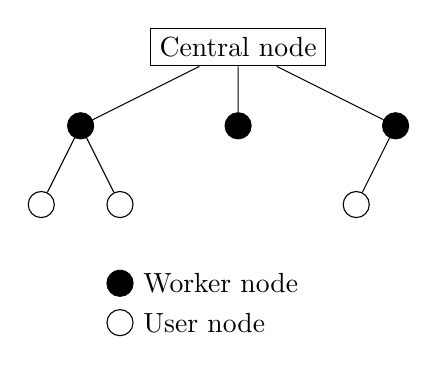
\begin{tikzpicture}

\node[draw] (C) at (0,0) {Central node};

\node[draw,style=circle,fill=black] (D1) at (-2,-1) {};
\node[draw,style=circle,fill=black] (D2) at (0,-1) {};
\node[draw,style=circle,fill=black] (D3) at (2,-1) {};

\draw[-] (C) -- (D1) (C) -- (D2) (C) -- (D3);

\node[draw,style=circle] (N1) at (-2.5,-2) {};\node[draw,style=circle] (N2) at (-1.5,-2) {};
\node[draw,style=circle] (N3) at (1.5,-2) {};

\draw[-] (N1) -- (D1) (N2) -- (D1) (N3) -- (D3);

\node[draw,style=circle,fill=black,label=right:Worker node] (L1) at (-1.5,-3) {};
\node[draw,style=circle,label=right:User node] (L2) at (-1.5,-3.5) {};

\end{tikzpicture}}
\end{center}
\caption{Distributed location proof system}
\label{fig:distributed_location}
\end{figure}

I consider a decentralised location proof system to be one where no node is in charge of controlling or coordinating the system. Nodes can create and publish location proofs between themselves, without the need for a central third party to coordinate the interaction (figure \ref{fig:decentralised_location}).

\begin{figure}[H]
\begin{center}
\resizebox {0.6\columnwidth} {!} {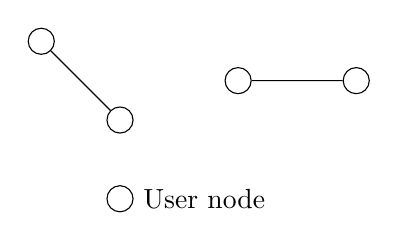
\begin{tikzpicture}

\node[draw,style=circle] (N1) at (-2.5,-1) {};\node[draw,style=circle] (N2) at (-1.5,-2) {};

\node[draw,style=circle] (N3) at (0,-1.5) {};
\node[draw,style=circle] (N4) at (1.5,-1.5) {};

\draw[-] (N1) -- (N2) (N3) -- (N4);

\node[draw,style=circle,label=right:User node] (L1) at (-1.5,-3) {};

\end{tikzpicture}}
\end{center}
\caption{Decentralised location proof system}
\label{fig:decentralised_location}
\end{figure}

\section{Existing location proof systems} \label{ssec:proof_systems}
Location proof systems are expected to be accurate and tamper-proof. For this reason, existing solutions have chosen to use a central authority to issue proofs, or to regulate proof issuance \cite{brassil, luo, khan}.

A hardware technique \cite{brassil}, developed by Brassil et al. of HP Laboratories, operates by supplementing existing WiFi access points (\textit{AP's}) with \textit{femtocells}. A femtocell is a small cellular antenna that connects to a mobile carrier via the Internet. Location verification over the internet is made possible by determining which femtocell a mobile node is connected to as it transfers data via Wi-Fi. This is possible because the central server in the location verification system has access to the mobile operator's user data. This solution requires investment in additional hardware to supplement existing WiFi access points, and requires access to mobile providers' user database to identify users locations (see figure \ref{fig:hp_labs}).

\begin{figure}[H]
\begin{center}
\resizebox {0.5\columnwidth} {!} {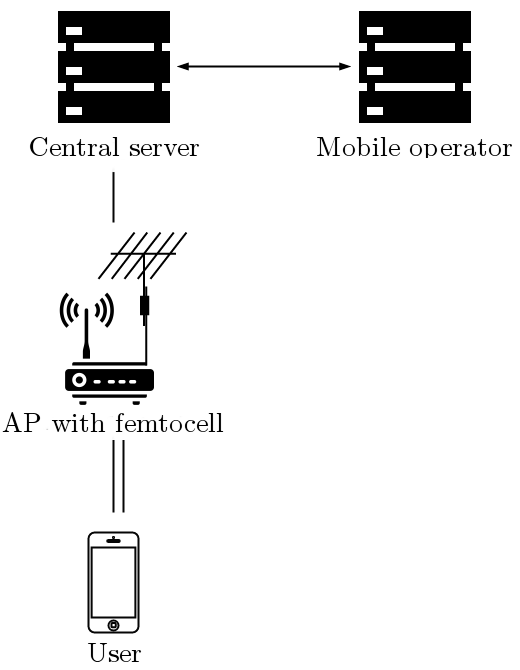
\includegraphics{diagrams/hp_paper.png}}
\caption{Hardware-based proof system (Adapted from Brassil et al. \cite{brassil})}
\label{fig:hp_labs}
\end{center}
\end{figure}

The use of a centralised system, as described above, creates security, privacy and vulnerability issues. An attacker who succeeds in compromising the security of the central server can violate the privacy of the users of the system, and potentially track their location. This is because in this system, location proofs reside with the central server, so the user has no control over their security. The central system architecture is also vulnerable, in the sense that a resource availability attack such as a DDoS attack could render the central architecture unavailable, making location verification unavailable.

Luo et al. propose a system that uses software installed on Wi-Fi access points to allow users to create location proofs \cite{luo}. In their system, each access point is given a \textit{group signature} by a central server, and can sign location proofs for users (figure \ref{fig:luo_diagram}).

\begin{figure}[H]
\begin{center}
\resizebox {0.5\columnwidth} {!} {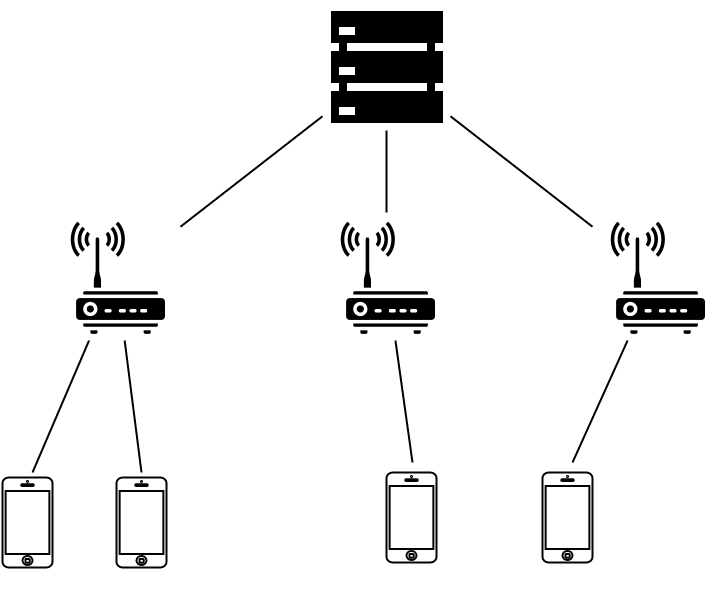
\includegraphics{diagrams/ap_paper.png}}
\caption{Access point proof system (Adapted from Luo et al. \cite{luo})}
\label{fig:luo_diagram}
\end{center}
\end{figure}

Users can request a location proof from any access point, and receive a proof encrypted by the AP with the group signature, as shown in figure \ref{fig:luo_transaction}. This can then be submitted to a Verifier.

This system creates \textit{proactive} location proofs. A proactive location proof is one which is created before it is needed. The user creates application-independent location proofs, and can use them at a later time with any application(s) he chooses.

A system proposed by Khan et al. takes a different approach, by using other users as witnesses to a location claim \cite{khan}. In this system, a \textit{witness} physically located near the user is used by the central server to verify the user's location claim (figure \ref{fig:witness_paper}). Like the model proposed by Luo et al., this system allows the user to have control over their own privacy, as the user owns the location proof.

\begin{figure}[H]
\begin{center}
\resizebox {0.4\columnwidth} {!} {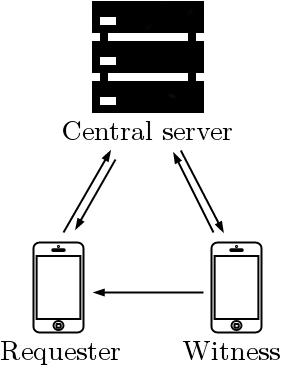
\includegraphics{diagrams/witness_paper.png}}
\caption{Proof system using witnesses (Adapted from Khan et al. \cite{khan})}
\label{fig:witness_paper}
\end{center}
\end{figure}

\section{Ad-hoc networks}

\section{Blockchain}

\section{Goals of a decentralised proof system}